\question

%% Use this if you have both Spanish and English versions
%% \ifspanish
%% % Here the Spanish version
%% \else
%% % Here the English version
%% \fi


Consider a detection problem with three hypothesis ($H \in\{0,1,2\}$) and observation $\mathbf{X} = (X_1, X_2)^T \in \mathbb{R}^2$. Moreover, we know that hypotheses are equally likely, also that
\begin{equation*}
  p_{X_1|X_2,H}(x_1|x_2,0) = p_{X_1|X_2,H}(x_1|x_2,1) = p_{X_1|X_2,H}(x_1|x_2,2),
\end{equation*}
and
\begin{align*}
  p_{X_2|H}(x_2|0) &= \begin{cases} 1/3, & |x_2| < 1.5, \\ 0, & \text{otherwise}, \end{cases} \\
  p_{X_2|H}(x_2|1) &= \begin{cases} x_2/2, & 0 < x_2 < 2, \\ 0, & \text{otherwise}, \end{cases}\\
  p_{X_2|H}(x_2|2) &= \begin{cases} -x_2/2, & -2 < x_2 < 0, \\ 0, & \text{otherwise}. \end{cases}
\end{align*}

Derive the decision regions of the detector that minimizes the probability of error.

\begin{solution}
   The detector that minimizes the probability of error is the maximum a posteriori detector, which is given by
   \begin{equation*}
      d = \arg \mathop{\operatorname{max}}_{h} P_{H|\mathbf{X}}(h|\mathbf{x}),
    \end{equation*}
    and can be rewritten as
   \begin{equation*}
      d = \arg \mathop{\operatorname{max}}_{h} p_{\mathbf{X}|H}(\mathbf{x}|h) P_H(h) = \arg \mathop{\operatorname{max}}_{h} p_{\mathbf{X}|H}(\mathbf{x}|h),
    \end{equation*}
    where the last step follows from $P_H(h) = 1/M$. However, we do not have the joint likelihood $p_{\mathbf{X}|H}(\mathbf{x}|h)$, but only $p_{X_1|X_2,H}(x_1|x_2,h)$ and $p_{X_2|H}(x_2|h)$. Using Bayes's theorem, the joint likelihood becomes
   \begin{equation*}
      p_{\mathbf{X}|H}(\mathbf{x}|h) = p_{X_1,X_2|H}(x_1,x_2|h) = p_{X_1|X_2,H}(x_1|x_2,h) p_{X_2|H}(x_2|h),
    \end{equation*}
    which yields
   \begin{align*}
      d &= \arg \mathop{\operatorname{max}}_{h} p_{\mathbf{X}|H}(\mathbf{x}|h) = \arg \mathop{\operatorname{max}}_{h} p_{X_1|X_2,H}(x_1|x_2,h) p_{X_2|H}(x_2|h) \\ &= \arg \mathop{\operatorname{max}}_{h} p_{X_2|H}(x_2|h),
    \end{align*}
    where, in the last step, we have taken into account that $p_{X_1|X_2,H}(x_1|x_2,h)$ does not depend on $h$. Then, the decision regions can only depend on $x_2$ and, to derive them, we need $p_{X_2|H}(x_2|h)$, which are plotted in the following figure
\begin{center}
		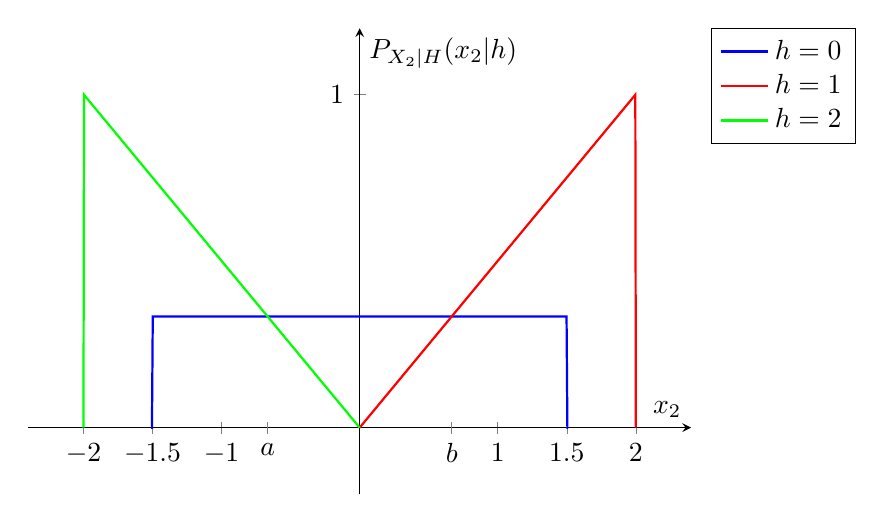
\begin{tikzpicture}
		\begin{axis}[%
		axis x line=middle,
		axis y line=middle,
		enlarge x limits=0.1,
		enlarge y limits=0.2,
		xtick={-2,-1.5,-1,0,1,1.5,2},
		%xticklabels={$-\pi$,$-\frac{2\pi}{N}$,$\frac{2\pi}{N}$,$\pi$},
		extra x ticks={-2/3,2/3},
		extra x tick labels={$a$,$b$},
		xmin=-2,
		xmax=2,
		ymin=0,
		%ytick=\empty,
		ytick={0,1},
		width=10cm,
		height=7.5cm,
		domain = -2:2,
		samples = 512,
		xlabel={$x_2$},
		ylabel={$P_{X_2|H}(x_2|h)$},
		legend pos=outer north east]
		\addplot[blue,thick,domain=-1.51:1.51] {1/3*(abs(x)<1.5)};
		\addlegendentry{$h = 0$};
		\addplot[red,thick,domain=0:2] {x/2*(x>0 && x<2)};
		\addlegendentry{$h = 1$};
		\addplot[green,thick,domain=-2:0] {-x/2*(x<0 && x>-2)};
		\addlegendentry{$h = 2$};
		\end{axis}
		\end{tikzpicture}
	\end{center}

    Hence, the decision regions, which are defined as 
  \begin{equation*}
    \mathcal{X}_d = \{\mathbf{x} | d = \arg \mathop{\operatorname{max}}_{h} p_{X_2|H}(x_2|h)\},
  \end{equation*}
  are given by
        \begin{equation*}
          \mathcal{X}_0 = \{x_2 \in \mathbb{R}  \mid a < x_2 < b \},
        \end{equation*}
        \begin{equation*}
          \mathcal{X}_1 = \{x_2 \in \mathbb{R}  \mid b \leq x_2 < 2 \},
        \end{equation*}
        and
        \begin{equation*}
          \mathcal{X}_2 = \{x_2 \in \mathbb{R}  \mid -2 < x_2 \leq a \}.
        \end{equation*}
        Hence, it remains to find the decision boundaries, which are the solution to
        \begin{equation*}
  P_{X_2|H}(b|0) = P_{X_2|H}(b|1) \Rightarrow b = \frac{2}{3},
\end{equation*}
and
\begin{equation*}
  P_{X_2|H}(a|0) = P_{X_2|H}(a|2) \Rightarrow a = -\frac{2}{3},
\end{equation*}
yielding
        \begin{equation*}
          \mathcal{X}_0 = \{x_2  \in \mathbb{R} \mid -2/3 < x_2 < 2/3 \},
        \end{equation*}
        \begin{equation*}
          \mathcal{X}_1 = \{x_2  \in \mathbb{R} \mid 2/3 \leq x_2 < 2 \},
        \end{equation*}
        and
        \begin{equation*}
          \mathcal{X}_2 = \{x_2  \in \mathbb{R} \mid -2 < x_2 \leq -2/3 \}.
        \end{equation*}
        
\end{solution}



